% Name: Beta decay
% Description: A neutron turning into a proton: one down quark becomes an up quark by emitting a W⁻ boson, which decays to an electron and an electron antineutrino.
% Tags: beta decay, weak interaction, W boson, neutron

\usepackage[compat=1.1.0]{tikz-feynman}

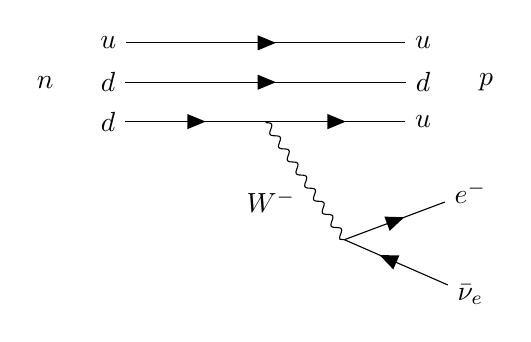
\begin{tikzpicture}
  \begin{feynman}
    \vertex (d1) at (0,0) {$d$};
    \vertex (a) at (2,0);
    \vertex (u1) at (4,0) {$u$};
    \vertex (d2) at (0,0.5) {$d$};
    \vertex (d3) at (4,0.5) {$d$};
    \vertex (u2) at (0,1) {$u$};
    \vertex (u3) at (4,1) {$u$};
    \vertex (b) at (3,-1.5);
    \vertex (e) at (4.6,-0.9) {$e^-$};
    \vertex (nu) at (4.6,-2.2) {$\bar\nu_e$};
    \diagram* {
      (d1) -- [fermion] (a) -- [fermion] (u1),
      (d2) -- [fermion] (d3),
      (u2) -- [fermion] (u3),
      (a) -- [boson, edge label'=$W^-$] (b),
      (b) -- [fermion] (e),
      (b) -- [anti fermion] (nu),
    };
  \end{feynman}
  \node at (-0.8,0.5) {$n$};
  \node at (4.8,0.5) {$p$};
\end{tikzpicture}
